\documentclass{news}
\usepackage{tikz}
\usetikzlibrary{arrows.meta,positioning}

\lang     {english}
\title    {The Ai Times:}
\subtitle {News, rumors, revelations, and prophecies from the age of artificial intelligence.}
\authors  {Alshival}
\keywords {newspaper, stories, journalism}
\date     {\today}
\location {Universal}
\cost     {}
\issue    {1}
\volume   {7}

\begin{document}

\by{Samuel Cavazos}{Top 100 Data \& Analytics Professional}{media/ait.png}

\hh{Large Language Regression Models}

{\l{L}ast year, a medical institution reached out to me with a very unique problem. They had a program that provided funding to undergraduate students conducting medical research. Students would submit a research proposal, and a review committee composed of some of the world's best medical researchers would evaluate the submissions. The problem was that members of the review committee are paid for their time, and the number of applications made a full manual review financially impossible. How could they efficiently evaluate all the proposals without overspending on reviewer compensation?
\par}

Their researchers had tried to use large language models for this task, hoping that the models could help evaluate the research proposals and reduce the burden on human reviewers. However, they found results were inconsistent and unreliable. I spoke with them about how large language models are designed for \emph{sequence-to-sequence} tasks rather than a \emph{regression} task like scoring research proposals, and the institution contracted me to do some research and see how far we could get.

They sent over a bunch of PDF files, so I had to do some preprocessing to extract the data. That was surprisingly difficult because college students. Some students used non-standard encodings, so when I extracted the text, the data was corrupted. Others submitted images of their proposal. That one made me laugh. The students would scan a printed hard-copy of their proposal and submit the scans in a PDF. In that case, text extraction fails because the PDF is essentially an image with no underlying text. I ended up having to use optical character recognition to get the text out of those image-based PDFs.

Once I had the training data, I spent a few weeks thinking about how to proceed. I had all this text. What could I do with it?

After a few hours at a whiteboard, I sketched out a plan for a class of models I now refer to as \emph{\textbf{large-language regression models}} (LLRMs). It was perfect for this kind of \emph{sequence-to-number} task.

\hh{The Four-Tensor Twist}

The initial LLRM I designed was based on the transformer architecture, with a twist. Instead of a single input tensor, I had four tensors of different dimensions. The \emph{title tensor} was an embedding of the project title. The \emph{abstract summary tensor} was another embedding, constructed by embedding the entire abstract at once. These are 1-dimensional tensors. In addition, I had two 2-dimensional tensors that had to be blended into the same architecture. Instead of embedding the abstract entirely, each sentence was embedded and the collection of these embeddings formed the \emph{abstract-sentence tensor}, a matrix of up to 50 sentence embeddings, each with 3,072 dimensions. Similarly, embedding each sentence of the proposal produced the \emph{proposal-sentence tensor}, a matrix of up to 512 sentence embeddings, each with 3,072 dimensions.

\hh{Blending the Four Tensors}
To combine the four tensors, I designed separate branches for each input. The title and abstract tensors went through dense layers to reduce their dimensionality. The abstract-sentence and proposal-sentence tensors went through positional encoding, transformer encoders, and attention pooling to produce fixed-length vectors. Finally, the outputs of all four branches were concatenated and fed into a regression head to produce the final score.

The model took about 6 to 12 hours to train on my RTX 4080. I remember laughing when I saw the results. 86\% of the test data was accurately classified when we used a threshold to determine whether an application makes the shortlist. I was curious though how it would do on completely new applications.

Well, they tried it last year, and results were so good that the client asked us to retrain the model for this year's set of applications. This past weekend, we trained on an RTX 5070 and were able to get up to 90\% accuracy on the test set. I had one of my data science interns do most of the heavy lifting this time so that they can take over the model next year.

LLRMs do not have the generative capabilities of LLMs; they are designed purely for producing a numerical score from text inputs rather than generating new sequences of text and that is what they excel at. An important model class that gets very little attention compared to LLMs, but has significant practical value in tasks involving evaluation, scoring, and filtering of text. The next time a sequence-to-number project lands on my desk, I will be ready.

\begin{center}
\resizebox{\linewidth}{!}{%
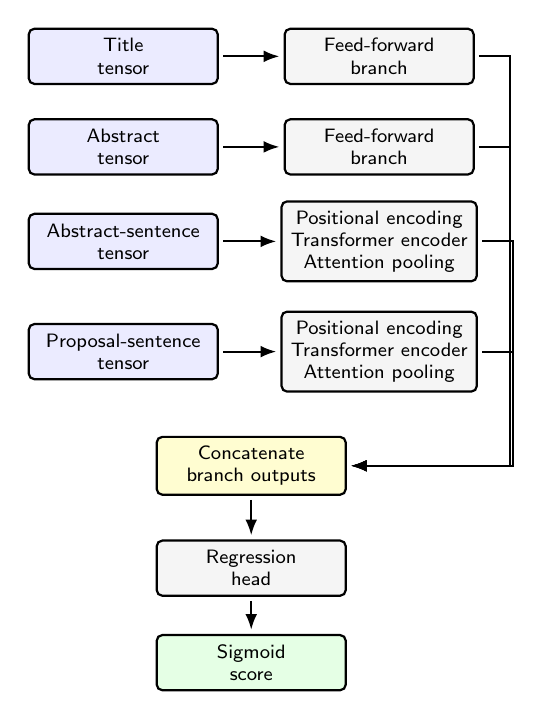
\begin{tikzpicture}[
    font=\sffamily\scriptsize,
    >=Latex,
    block/.style={draw, rounded corners=2pt, thick, align=center, minimum width=24mm, minimum height=7mm, fill=gray!8},
    input/.style={block, fill=blue!8},
    output/.style={block, fill=green!10},
    merge/.style={block, fill=yellow!18},
    arrow/.style={-{Latex[length=2mm,width=1.5mm]}, thick, shorten >=1.5pt, shorten <=1.5pt}
]
\node[input] (title) at (0, 0) {Title\\tensor};
\node[block] (titleff) at (3.25, 0) {Feed-forward\\branch};

\node[input] (abstract) at (0, -1.15) {Abstract\\tensor};
\node[block] (abstractff) at (3.25, -1.15) {Feed-forward\\branch};

\node[input] (abstractsent) at (0, -2.35) {Abstract-sentence\\tensor};
\node[block] (abstractpath) at (3.25, -2.35) {Positional encoding\\Transformer encoder\\Attention pooling};

\node[input] (proposal) at (0, -3.75) {Proposal-sentence\\tensor};
\node[block] (proposalpath) at (3.25, -3.75) {Positional encoding\\Transformer encoder\\Attention pooling};

\node[merge] (concat) at (1.625, -5.2) {Concatenate\\branch outputs};
\node[block] (head) at (1.625, -6.5) {Regression\\head};
\node[output] (score) at (1.625, -7.7) {Sigmoid\\score};

\draw[arrow] (title) -- (titleff);
\draw[arrow] (abstract) -- (abstractff);
\draw[arrow] (abstractsent) -- (abstractpath);
\draw[arrow] (proposal) -- (proposalpath);

\draw[arrow] (titleff.east) -- ++(0.45,0) |- (concat.east);
\draw[arrow] (abstractff.east) -- ++(0.45,0) |- (concat.east);
\draw[arrow] (abstractpath.east) -- ++(0.45,0) |- (concat.east);
\draw[arrow] (proposalpath.east) -- ++(0.45,0) |- (concat.east);
\draw[arrow] (concat.south) -- (head.north);
\draw[arrow] (head.south) -- (score.north);
\end{tikzpicture}%
}

{\scriptsize Schematic of the full four-branch LLRM architecture.}
\end{center}

\hh{Announcements}

\textit{The Ai Times} is now on Substack. Scan the code below to get each new issue, along with the sources, side quests, and stray prophecies that did not fit on the page.

\begin{minipage}[c]{.50\linewidth}
{\large\cinzel
{\normalsize The }

\qquad Ai

\qquad\quad Times}
\end{minipage}%
\begin{minipage}[c]{0.50\linewidth}

\includegraphics[width=\linewidth]{media/ai-times-qr.png}
\end{minipage}

\end{document}
